\documentclass[11pt]{article}
\usepackage{fullpage}
\usepackage{algorithm}
\usepackage[noend]{algorithmic}
\usepackage{enumerate}
\usepackage{amsmath,amssymb,amsthm}
\usepackage{stackrel}
\usepackage{tikz}

\usepackage{caption}

\DeclareCaptionType{mytype}[Diagram][List of mytype]
\newenvironment{myenv}{}{}

% Helpful Shortcuts
\newcommand{\bc}[1]{{\quad \text{(#1)}}} 	% Justification in math env
\newcommand{\st}{{\text{ such that }}} 							   % Math env
\newcommand{\abs}[1]{{ |#1 |}} 							% Absolute value / Cardinality
\newcommand{\bld}[2]{\noindent\textbf{#1:}\hspace{0.1in}#2$  $\bigskip} % Headings
\newcommand{\notimplies}{%
	\mathrel{{\ooalign{\hidewidth$\not\phantom{=}$\hidewidth\cr$\implies$}}}}
\newcommand{\linesep}{\noindent\bigskip\rule{17cm}{0.1mm}\bigskip} % Horizontal Line

% These define new environments / formats for lemmas, definitions, running time, etc.
\newtheorem{lemma}{Lemma}
\newtheorem{definition}{Definition}
\newtheorem{notation}{Notation}
\newtheorem*{claim}{Claim}
\newtheorem{observation}{Observation}
\newtheorem{conjecture}[lemma]{Conjecture}
\newtheorem{theorem}[lemma]{Theorem}
\newtheorem{corollary}[lemma]{Corollary}
\newtheorem{proposition}[lemma]{Proposition}
\newtheorem*{rt}{Running Time}

% These define nice ways to format P and OPT (use \P or \opt)
\def\P{\ensuremath{$ \mathcal{P} $}}
\def\opt{\ensuremath{\textsc{opt}}}
\renewcommand{\labelenumi}{\bf \alph{enumi}.}

\renewcommand\maketitle{
	\begin{center}
		\begin{tabular*}{6.44in}{l @{\extracolsep{\fill}}c r}
			\bfseries  &  & \bfseries CSCI 383 Spring 2019 \\
			\bfseries&  & \bfseries  Homework \#8 Solutions  \\
			\bfseries   &   &  \bfseries Kai Ting Keshia Yap\\ 
		\end{tabular*}
\end{center} }

\begin{document}
	\maketitle
	
	\noindent Honor Code: I affirm that I adhered to the Honor Code in this assignment. Keshia Yap\\
	
	
	\subsection*{Part 1: Power Move}
%	Give a Turing machine that accepts the language $ \{a^{2^n}\mid n\geq 0\}  $
%	Your solution should include:
%	Your solution should include:\\
%	1. An informal description of the Turing machine.\\
%	2. A formal description, including all transitions.\\
	
%	For stating the transitions, I would recommend either a table such as the one on page 212 of Kozen, or a flowchart-like diagram such as the ones we used for DFAs, with nodes for states, and for each transition $ ((p, b),(q, c, d)) $, label the arrow from state $ p $ to state $ q $ with the triple $ (b, c, d) $. However you decide to present your machine, make sure it is clear what labeling system you are using.

	Let $ M=(Q,\Sigma,  \Gamma, \vdash, \textvisiblespace,\delta, s, t, r)  $ be a Turing machine where 
	\begin{itemize}
		\item $ Q=\{s,t,r,c,q_0,q_1,q_2\} $
		\item $ \Sigma =\{a\} $
		\item $ \Gamma = \{\vdash, \dashv, \textvisiblespace, a, \hat{a} \} $
		\item $ \delta $ transitions are shown in Diagram 1, where arrows from state $ p $ to state $ q $ with the triple $ (b, c, d) $ represent the transition $ ((p, b),(q, c, d)) $. 
%		Transitions not shown are not important.
	\end{itemize}

	\begin{center}
%	\begin{figure}
		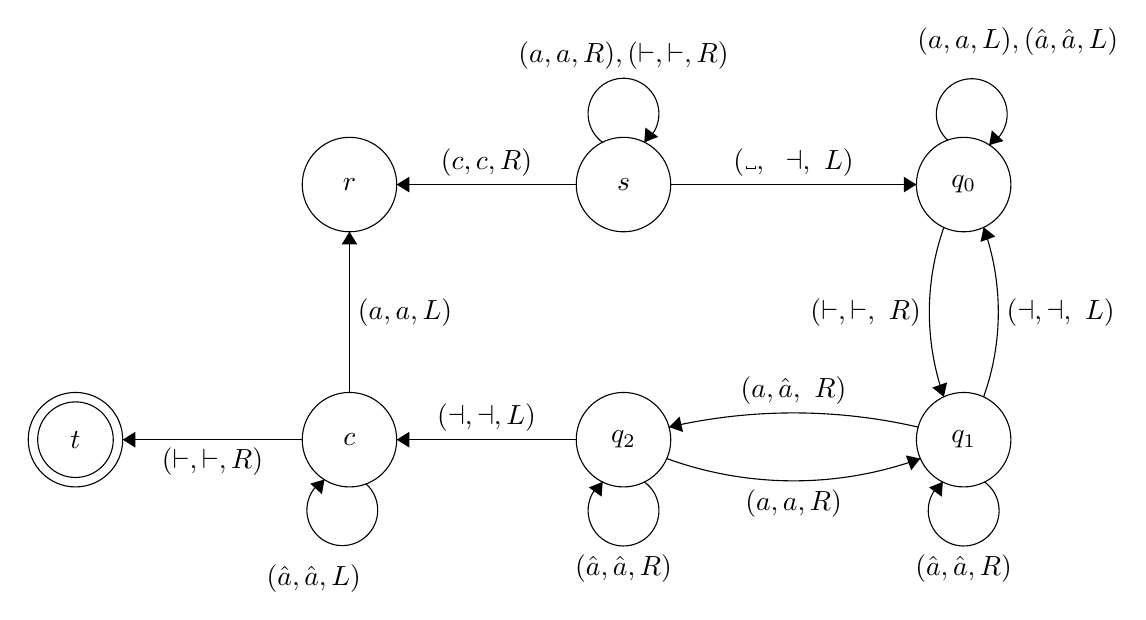
\begin{tikzpicture}[scale=0.2]
		\tikzstyle{every node}+=[inner sep=0pt]
		\draw [black] (39.4,-12.3) circle (3);
		\draw (39.4,-12.3) node {$s$};
		\draw [black] (61,-12.3) circle (3);
		\draw (61,-12.3) node {$q_0$};
		\draw [black] (61,-28.5) circle (3);
		\draw (61,-28.5) node {$q_1$};
		\draw [black] (39.4,-28.5) circle (3);
		\draw (39.4,-28.5) node {$q_2$};
		\draw [black] (22,-28.5) circle (3);
		\draw (22,-28.5) node {$c$};
		\draw [black] (4.6,-28.5) circle (3);
		\draw (4.6,-28.5) node {$t$};
		\draw [black] (4.6,-28.5) circle (2.4);
		\draw [black] (22,-12.3) circle (3);
		\draw (22,-12.3) node {$r$};
		\draw [black] (42.4,-12.3) -- (58,-12.3);
		\fill [black] (58,-12.3) -- (57.2,-11.8) -- (57.2,-12.8);
		\draw (50.2,-11.8) node [above] {$(\textvisiblespace,\mbox{ }\dashv,\mbox{ }L)$};
		\draw [black] (59.744,-25.78) arc (-160.5294:-199.4706:16.142);
		\fill [black] (59.74,-25.78) -- (59.95,-24.86) -- (59.01,-25.19);
		\draw (58.32,-20.4) node [left] {$(\vdash,\vdash,\mbox{ }R)$};
		\draw [black] (42.291,-27.701) arc (103.00307:76.99693:35.152);
		\fill [black] (42.29,-27.7) -- (43.18,-28.01) -- (42.96,-27.03);
		\draw (50.2,-26.3) node [above] {$(a,\hat{a},\mbox{ }R)$};
		\draw [black] (36.4,-28.5) -- (25,-28.5);
		\fill [black] (25,-28.5) -- (25.8,-29) -- (25.8,-28);
		\draw (30.7,-28) node [above] {$(\dashv,\dashv,L)$};
		\draw [black] (19,-28.5) -- (7.6,-28.5);
		\fill [black] (7.6,-28.5) -- (8.4,-29) -- (8.4,-28);
		\draw (13.3,-29) node [below] {$(\vdash,\vdash,R)$};
		\draw [black] (22,-25.5) -- (22,-15.3);
		\fill [black] (22,-15.3) -- (21.5,-16.1) -- (22.5,-16.1);
		\draw (22.5,-20.4) node [right] {$(a,a,L)$};
		\draw [black] (38.077,-9.62) arc (234:-54:2.25);
		\draw (39.4,-5.05) node [above] {$(a,a,R),(\vdash,\vdash,R)$};
		\fill [black] (40.72,-9.62) -- (41.6,-9.27) -- (40.79,-8.68);
		\draw [black] (59.993,-9.486) arc (227.41806:-60.58194:2.25);
		\draw (64.44,-4.13) node [above] {$(a,a,L),(\hat{a},\hat{a},L)$};
		\fill [black] (62.62,-9.79) -- (63.53,-9.54) -- (62.79,-8.86);
		\draw [black] (62.323,-31.18) arc (54:-234:2.25);
		\draw (61,-35.75) node [below] {$(\hat{a},\hat{a},R)$};
		\fill [black] (59.68,-31.18) -- (58.8,-31.53) -- (59.61,-32.12);
		\draw [black] (40.723,-31.18) arc (54:-234:2.25);
		\draw (39.4,-35.75) node [below] {$(\hat{a},\hat{a},R)$};
		\fill [black] (38.08,-31.18) -- (37.2,-31.53) -- (38.01,-32.12);
		\draw [black] (23.044,-31.3) arc (48.17063:-239.82937:2.25);
		\draw (19.73,-36.38) node [below] {$(\hat{a},\hat{a},L)$};
		\fill [black] (20.41,-31.03) -- (19.51,-31.29) -- (20.25,-31.96);
		\draw [black] (62.268,-15.014) arc (19.66917:-19.66917:16.002);
		\fill [black] (62.27,-15.01) -- (62.07,-15.94) -- (63.01,-15.6);
		\draw (63.7,-20.4) node [right] {$(\dashv,\dashv,\mbox{ }L)$};
		\draw [black] (58.252,-29.699) arc (-70.05613:-109.94387:23.607);
		\fill [black] (58.25,-29.7) -- (57.33,-29.5) -- (57.67,-30.44);
		\draw (50.2,-31.62) node [below] {$(a,a,R)$};
		\draw [black] (36.4,-12.3) -- (25,-12.3);
		\fill [black] (25,-12.3) -- (25.8,-12.8) -- (25.8,-11.8);
		\draw (30.7,-11.8) node [above] {$(c,c,R)$};
		\end{tikzpicture}
%		\caption{M1} \label{States and transitions in Turing machine $ M $}
%\end{figure}
		\begin{myenv}
			\captionof{mytype}{States and transitions in Turing machine $ M $}
		\end{myenv}
	\end{center}

		Informally, the Turing machine works in the following way:
		
		\begin{algorithm}
		\textbf{Algorithm PowerOfTwo$ (M, x) $}
		\begin{algorithmic}
			\STATE loop through $ x $
			\IF{there exists some $ c\neq a $ in $ x $}
			\RETURN reject
			\ENDIF
			\STATE find the first blank space character and replaces it with an $ \dashv $ character
			\WHILE{the $ a $ immediately before $ \dashv $ is unmarked}
			\STATE move finite control to $ \vdash $
			\WHILE{the character read is not $ \dashv $}
			\STATE mark every other $ a $ with a hat ($ \hat{a} $), ignoring the pre-existing $ \hat{a} $s
			\ENDWHILE
			\ENDWHILE
			\IF{there exists some unmarked $ a $s on the tape}
			\RETURN reject 
			\ENDIF
			\RETURN accept
		\end{algorithmic}
		\end{algorithm}
	
		\begin{enumerate}[1.]
			\item Check if there the string contains some non-$ a $ character (states $ s, r $). If so, reject.
			\item Taper the end of the string with a $ \dashv $ character (state $ s  $ to $ q_0 $).
			\item Return the finite control to the $ \vdash $ character on the left (state $ q_0 $).
			\item Sweep right, repeatedly marking every other $ a $, ignoring $ \hat{a} $s (i.e. half of the existing $ a $s) (states $ q_1,q_2 $).
			\item If we mark an $ a $ that is right before the $ \dashv $ character, we move into the checking state $ c $.
			\item Sweep left to check if the entire string of $ a $'s are marked. Accept if this is true, reject otherwise.
		\end{enumerate}

	\begin{claim}
		$ M $ accepts exactly the language $ \{a^{2^n}\mid n\geq 0 \} $:		
	\end{claim}
	\begin{proof}
		Since the machine $ M $ marks every other $ a $ from the left to the right, if we mark some $ a $ that is right before the $ \dashv $ symbol, it means that there was an odd number of $ a $'s on that sweep. That is, the number of $ a $'s had an odd factor, and so cannot be a power of $ 2 $. Otherwise, if that $ a $ was the only one left unmarked, then the number of $ a $'s is a power of $ 2 $ (since the number of $ a $'s were repeatedly divided by two, to get 1).
	\end{proof}
\end{document}